\section{Einleitung}
Vor allem im 21. Jahrhundert wird Umweltfreundlichkeit immer wichtiger. Immer mehr Menschen fahren deshalb und aus vielen anderen Gründen (Gesundheit, Zeitersparnis, etc…) mit dem Fahrrad \cite{}. In vielen engen (und immer enger werdenden \cite{}) Großstädten der Welt ist das sichere Lagern von Fahrrädern jedoch schwierig bis unmöglich. Herkömmliche Fahrradständer sind zwar platzeffizient und billig, jedoch nicht sicher \cite{}. Besonders bei teuren E-Bikes traut sich mancher nicht, dieses einfach an einen Pfosten zu sperren. Als Alternative dazu gibt es Rad-Boxen oder unterirdische Garagen, beide Optionen sind aber teurer, eingeschränkt nutzerfreundlich und oft zu weit weg von dem Ort, an dem man hinwill.

\begin{figure}[ht]
  \centering
  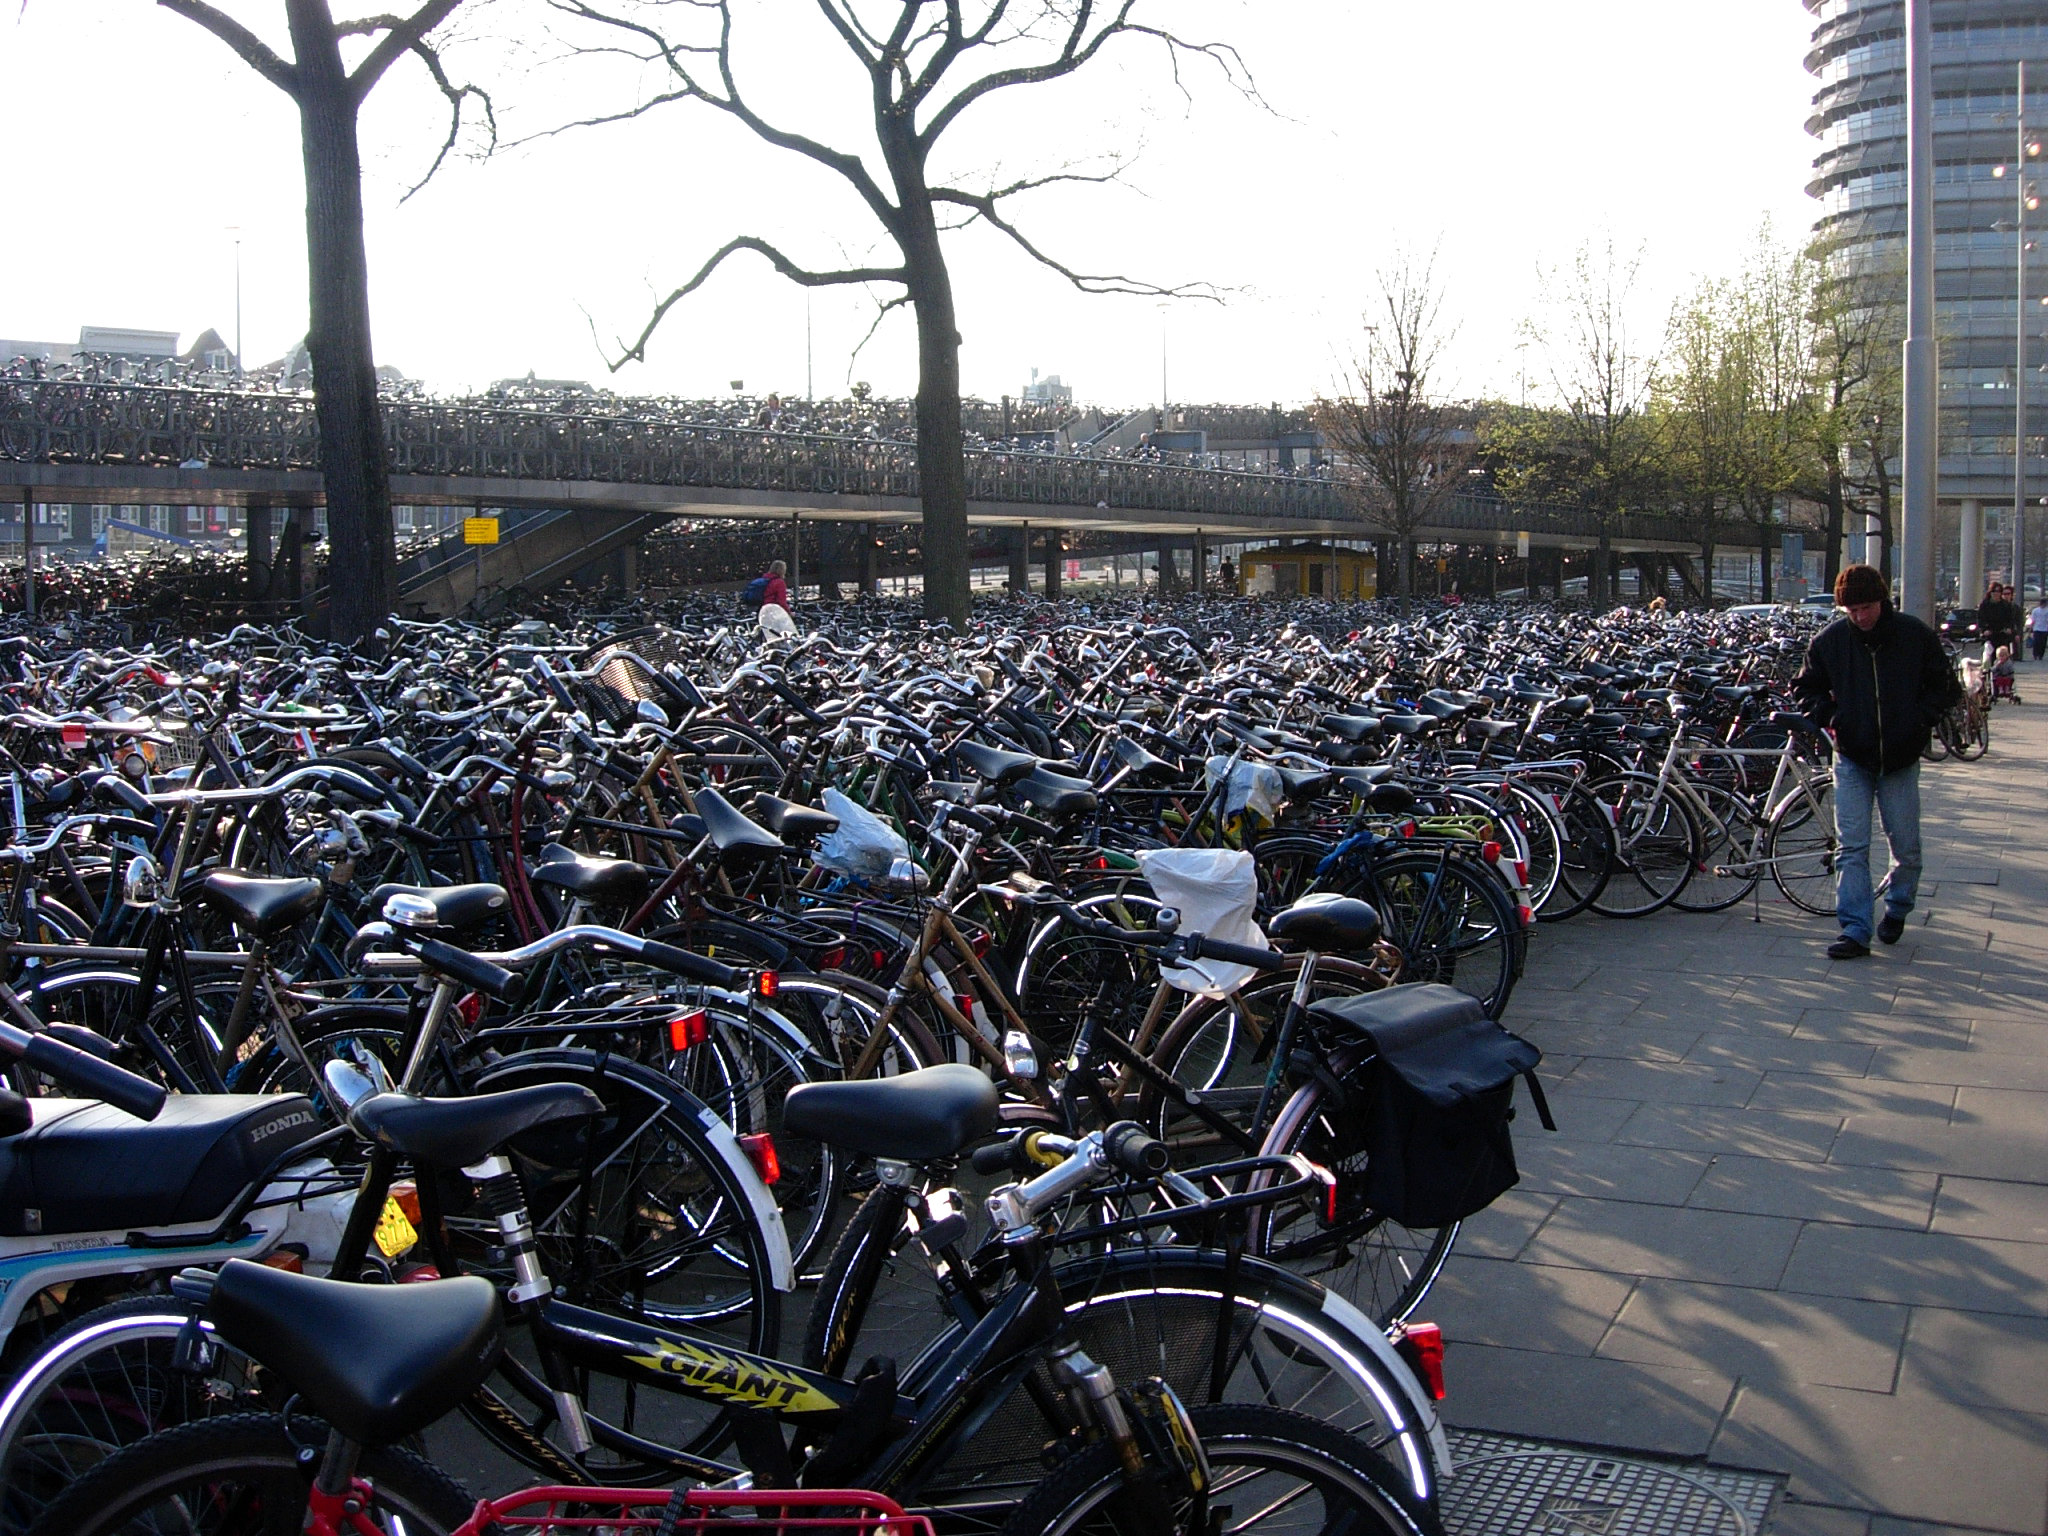
\includegraphics[width=0.5\textwidth]{images/fahrrad_parkhaus_voll}
  \caption{Randvolles Fahrrad-Parkhaus in Amsterdam (CC Jakub Hałun \cite{cc})}
  \label{fig:fahrrad_parkhaus_voll}
\end{figure}

In Zukunft wird es sogar noch mehr E-Bikes geben, denn fast die Hälfte aller verkauften Fahrräder sind mit Elektroantrieb ausgestattet (Tendenz stark steigend) \cite{}. Vor allem der urbane Raum benötigt derzeit dringend Abstellmöglichkeiten, wo Fahrräder schnell, sicher und möglichst billig in der Nähe geparkt werden können.

\subfile{entstehung_der_idee.tex}

\subfile{problemstellung.tex}

\subfile{zielsetzung.tex}
